

\section{Recontrucción}


\subsubsection{Introducción}

A la salida del bloque de detección de marcadores se tiene,  para cada cámara y para cada frame de una secuencia adquirida, un conjunto de coordenadas en dos dimensiones $(x,y)$ que ubican la posición en la imagen de aquellos marcadores que fueron detectados. 
El proceso de reconstrucción consiste en obtener las coordenadas en tres dimensiones de la posición de los marcadores en el espacio a partir de  las coordenadas en dos dimensiones obtenidas en el bloque anterior.
En la figura \ref{fig: esquema_reconstruccion} se muestra un ejemplo de reconstrucción para el caso de dos cámaras.\\


\begin{figure}[h!]
\begin{center}
\includegraphics[scale=0.25]{img/Reconstruccion/ejemplo_reconstruccion1.png}
\end{center}
\caption{Reconstruccion con dos camaras}
\label{fig: esquema_reconstruccion}
\end{figure}


Se observa en la figura a uno de los marcadores detectados desde las dos vistas y su correspondiente punto 3D reconstruido.\\

El proceso de reconstrucción implementado consiste en tres pasos fundamentales:


\begin{enumerate}
\item Determinar  aquellos marcadores detectados en las distintas cámaras que corresponden a un mismo marcador en el espacio. De esta manera se establece una correspondencia entre los marcadores detectados en las distintas vistas. Dichas asociaciones se establecen de a pares de cámaras.
\item Una vez establecidas estas correspondencias se selecciona aquella que con algún criterio pueda considerarse con mayores posibilidades de ser una asociación correcta. Luego se determina la posición en el espacio del marcador a partir de la asociación seleccionada.

\item Una vez reconstruido uno de los marcadores debe verificarse si dicho marcador fue detectado en el resto de las cámaras
\end{enumerate}

\begin{figure}[h!]
\begin{center}
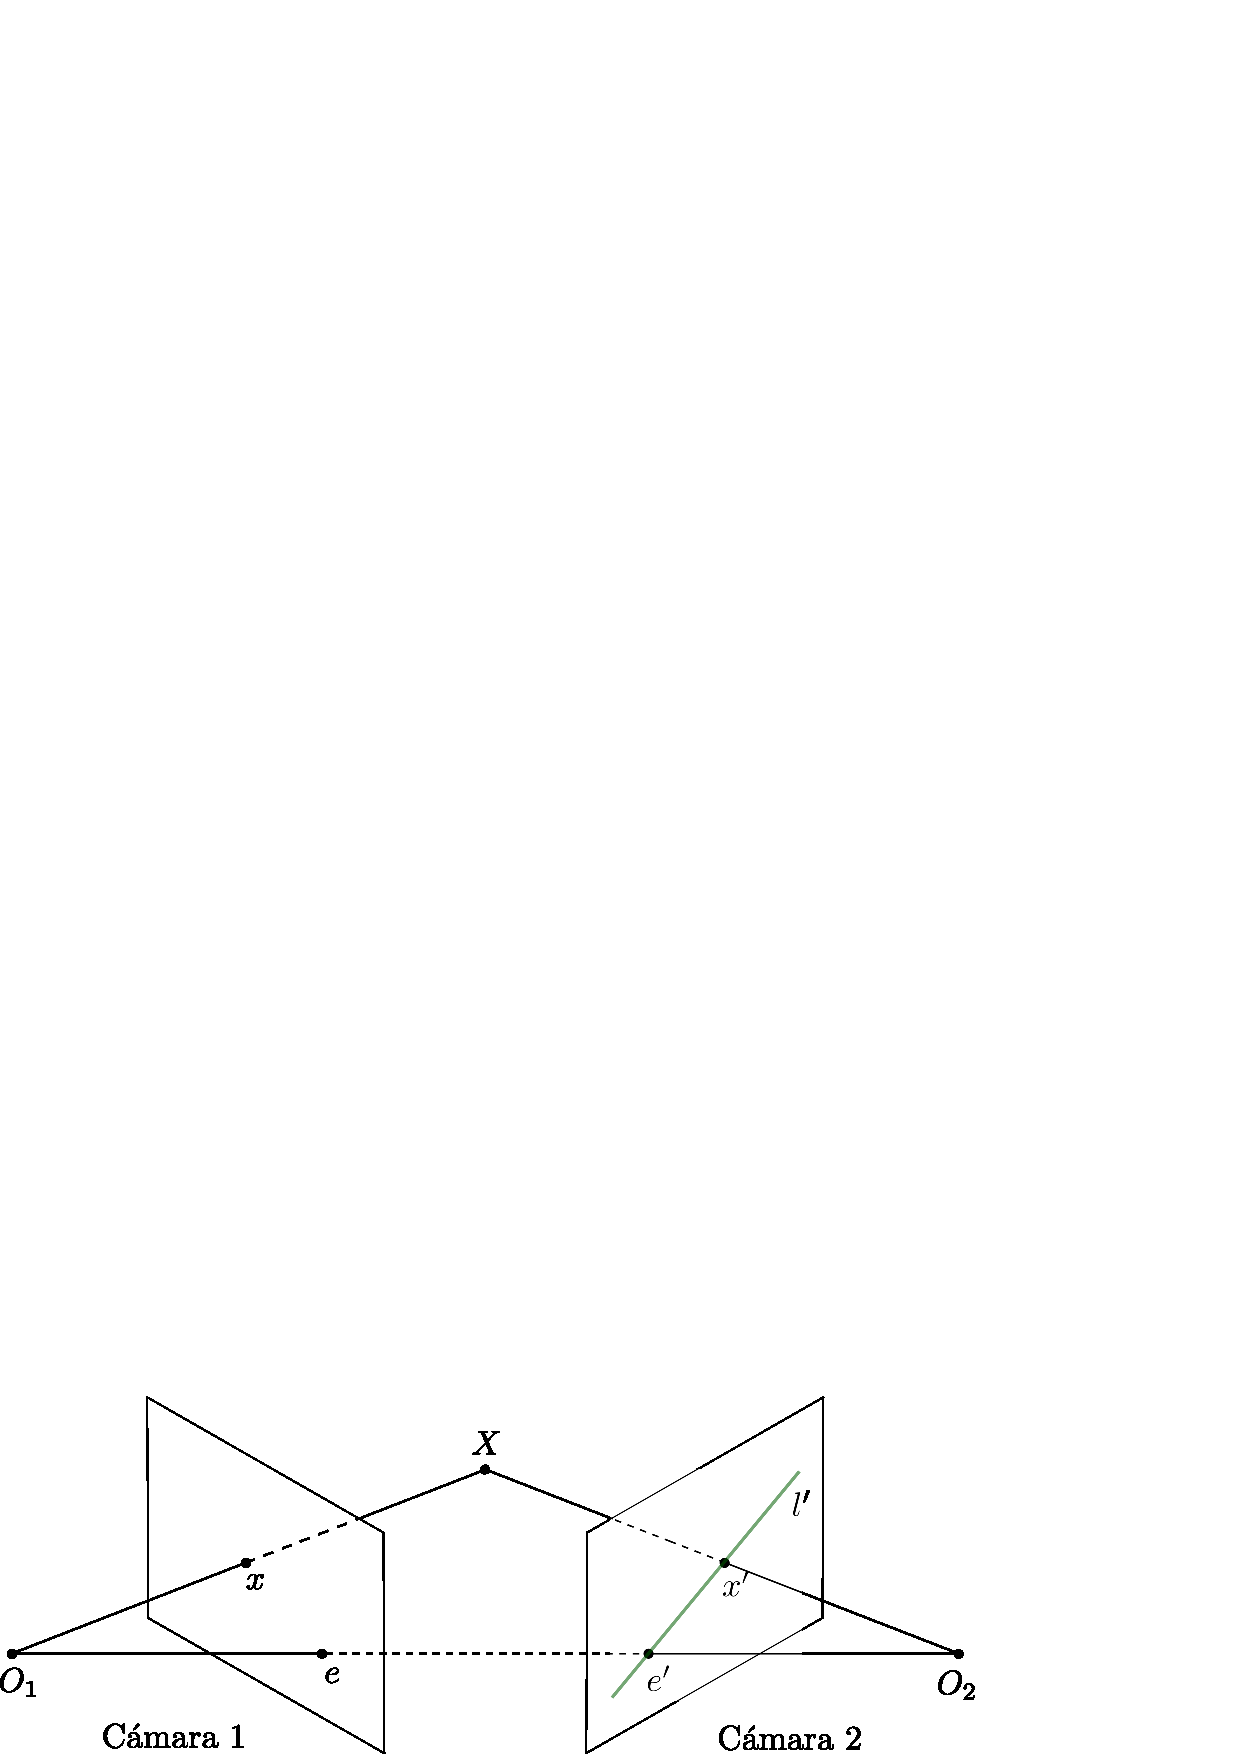
\includegraphics[scale=0.7]{img/Reconstruccion/geometria_epipolar.pdf}
\end{center}
\caption{Reconstruccion con dos camaras}
\label{fig: geometria_epipolar}
\end{figure}

Como se explicó anteriormente, se inicia la implementación de este bloque a partir del algoritmo propuesto por Herda \cite{Herda} para este caso. A este algoritmo se le hicieron cambios debido a interpretaciones rellizadas sobre aspectos del algoritmo que no han quedado del todo establecidas y a la evaluación de su rendimiento.\\



Dicha reconstrucción se realiza utilizando lo que se denomina triangulación estéreo \cite{Faugueras}, que utiliza las propiedades de la geometría epipolar. Como se muestra en la figura \ref{fig:geom_epipolar}, dadas dos cámaras y un punto 3D en el espacio \(X\), dicho punto se proyecta en dichas cámaras en los puntos \(x\) y \(x’\). Es decir, \(x\) pertenece a la intersección de la retina de la cámara 1, con la recta formada por el foco \(O_1\) y el punto \(X\). Análogamente se construye el punto \(x’\) de la cámara 2. A su vez, los focos de ambas cámaras \(O_1\) y \(O_2\) definen una recta  que corta a las retinas de las cámaras en los puntos \(e\) y \(e’\), llamados epipolos.

Por lo tanto se tiene que \(O_1,~O_2\) y \(X\) definen un plano, llamado plano epipolar. Dicho plano contiene además, los puntos \(x\), \(x’\), \(e\), \(e’\) y corta a la retina de cada cámara en una línea, que recibe el nombre de línea epipolar. La línea epipolar de la cámara 1, contiene a los puntos \(e\) y \(x\), y la de la cámara 2 a los puntos \(e’\) y \(x’\).
	
Para poder hacer la reconstrucción de los marcadores, en primer lugar debe hallarse para cada punto \(x\) proyectado en una cámara su correspondiente punto \(x’\) en otra cámara. De lo visto anteriormente, un punto \(x\) en la cámara 1 y los focos de ambas cámaras definen un plano que corta a la retina de la cámara 2 en la línea epipolar \(l'\) que contiene a su correspondiente punto \(x’\) en la cámara 2. Por lo tanto, para establecer esa correspondencia, se encuentra para cada punto del conjunto de marcadores detectados de la cámara 1, la recta epipolar sobre la cámara 2 y se selecciona aquel punto detectado de esta cámara que esté contenido en dicha recta.

Debido a imperfecciones de las cámaras, la proyección real de un punto 3D va a ser aproximadamente el punto ideal de su proyección. 
